%% This is an example first chapter.  You should put chapter/appendix that you
%% write into a separate file, and add a line \include{yourfilename} to
%% main.tex, where `yourfilename.tex' is the name of the chapter/appendix file.
%% You can process specific files by typing their names in at the 
%% \files=
%% prompt when you run the file main.tex through LaTeX.
\chapter{Introduction}\label{intro-ch}

\section{Spark and MapReduce}


New data processing systems such as Spark and MapReduce have been designed to help process the increasing amount of data \cite{MapReduce} \cite{Sparkfull}. 
Instead of relying on just one powerful computer, these systems use many computers due to lower costs, increased scalability, and improved fault tolerance. 
Because these systems are distributed in nature, they have stages (shuffle stages) where they transfer information between computers. 
\section{Shuffle} 

We will use MapReduce to explain the shuffle in more detail, but the main concepts still apply to Spark.

\subsection{Shuffle Introduction}
In the first stage of MapReduce, the map phase, the data is loaded onto different computers and computation is performed on it that results 
in a group of key-value pairs. The final phase of MapReduce, the reduce phase, assumes that all key-value pairs with the same
key are grouped together onto the same machine. We call this property the shuffle guarentee. Thus, the shuffle phase, an intermediate phase that the system handles internally, transfers key-value pairs between machines to satisfy the shuffle guarentee. 


Figure~\ref{fig:shuffle_basic} display the inner workings 
of the shuffle phase. For instance, a programmer may  want to count the 
number of letters in a distributed file. The mappers will each load part of the distributed file and count the number of
letters in their part. However, the systems needs to aggregate the count for each letter and 
thus all the counts for letter A will be sent to Reducer 1, letter B will be sent to Reducer 2,
and letter C will be sent to Reducer 3. These reducers will then promptly aggregate the counts that they receive from the 
mappers.

\begin{figure}[h]
\begin{center}
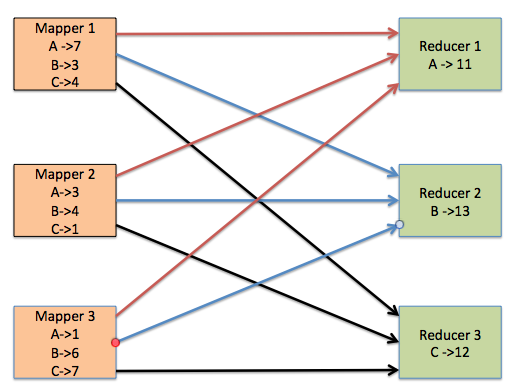
\includegraphics[scale=0.6]{./img/shuffle_basic.png}
\caption{Shuffle for Letter Count in MapReduce}
\label{fig:shuffle_basic}
\end{center}
This figures demonstrates a basic shuffle in MapReduce. 
Each mapper sends its letter counts to different reducers such that each reducer
gets the total letter count for a specific letter.
\end{figure}
Due to the huge amounts of keys, these systems do not transfer data on the granurality of keys.
Instead, they use partitions, which contain key-value pairs with different keys. Programmers can pick different partitioning functions such as hash partitiong and range partitiong to map keys to partitions. Two identical keys are guarenteed to be in the same partition. As long as all the mappers partition their data in the same way and send each partition with the same index to the same reducer, the system satisfies 
the shuffle guarentee. 

\subsection {Shuffle Analysis}

MapReduce is constrained by the slowest worker; therefore, minimizing the latency of the slowest worker should improve performance.
Balancing the amount of data sent to each reducer helps achieve this by reducing both network latency and also the execution time for the slowest worker.
Figure~\ref{fig:shuffle_unbalanced}, depicts a shuffle scenario that results in unbalanced paritions. A basic heuristic is used with each reducer getting half of the mapper output partitions. Generally, this protocol should result in  balanced reducers, but as seen, Reducer 2 receives 
twice the amount of data as Reducer 1. However, if the system knew the sizes of the map output partitions,
it could more intelligently balance the reducers. As seen in Figure~\ref{fig:shuffle_balanced}, with the same map output partitions, the system could attain complete balance
of 60MB for each reducer.


 \begin{figure}[h]
\begin{center}
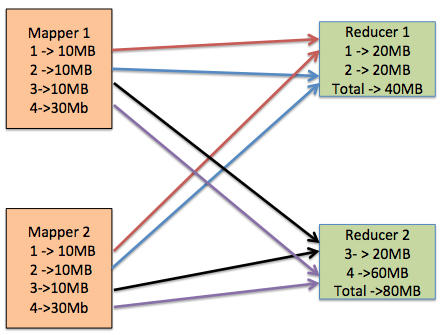
\includegraphics[scale=1.0]{./img/shuffle_unbalanced.png}
\caption{Unbalanced Shuffle} 
\label{fig:shuffle_unbalanced}
\end{center}
Reducer 1 requests partition 1 and 2 while Reducer 2 requests partition 3 and 4. 
This results in Reducer 2 receiving 80MB of data while Reducer 1 receives only 40MB of data. 
\end{figure}

 \begin{figure}[h]
\begin{center}
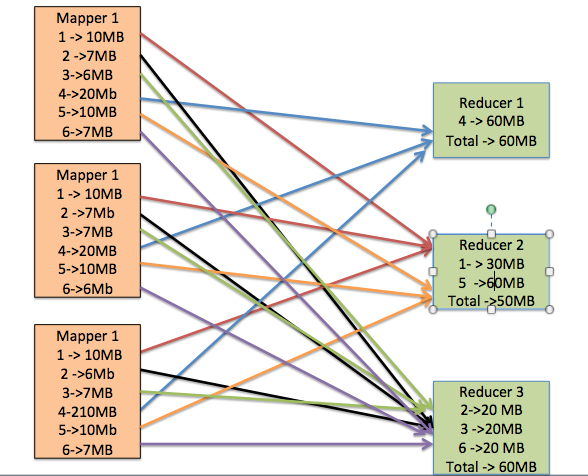
\includegraphics[scale=1.0]{./img/shuffle_balanced.png}
\caption{Balanced Shuffle}
\label{fig:shuffle_balanced}
\end{center}
\end{figure}

\section{Adaptive Scheduling of Joins}\label{intro-ch:eeg-overview}

\subsection{Join Basics}

A common operation in these data processing environments is a join \cite{join}.
A join basically combines two tables by finding intersections between
keys in respective columns. For instance, if we have   
Table \ref{table:join1} and Table \ref{table:join2} that we are trying to join based on the intersection
of key1 and key2, the resulting output is Table \ref{table:join3}   
\begin{table}[h!]
\centering
 \begin{tabular}{|c |c |c |c|}
  \hline
   Key1 & Value1 \\
  \hline
   a & 1 \\
  \hline
   a & 1 \\
  \hline
   b & 3 \\
  \hline
   c & 4 \\
  \hline
\end{tabular}
\caption{Table for Dataset 1}
\label{table:join1}
\end{table}

\begin{table}[h!]
\centering
 \begin{tabular}{|c |c|}
  \hline
   Key2 & Value2 \\
  \hline
   a & 5 \\
  \hline
   c & 7 \\
  \hline
\end{tabular}
\caption{Table for dataset 2}
\label{table:join2}
\end{table}

\begin{table}[h!]
\centering
 \begin{tabular}{|c |c |c|}
  \hline
   Key1 & Value1 & Value2  \\
  \hline
   a & 1 & 5 \\
  \hline
   a & 2 & 5 \\
  \hline
   c & 4 & 7 \\
  \hline
\end{tabular}
\caption{Table of Joined Data}
\label{table:join3}
\end{table}

\subsection{Shuffle Join}
The actual implementation of joins in MapReduce is very similar to the
shuffle scenario presented above. Instead of having output partitions for just one dataset,
the mappers have output partitions for two datasets and ensure that all partitions for both datasets with the same index 
are sent to the same reducer.  
Figure \ref{fig:shuffle_join} details a shuffle join.
For both datasets, all of the keys that 
mapped to partition 1 were sent to Reducer 1 and this happens respectively for the rest of the partitions. Because
all identical keys are in the same partition and each partition with the same index is sent to the same reducer,
the system is guarenteed to find all intersections required for the join.

\begin{figure}[h]
\begin{center}
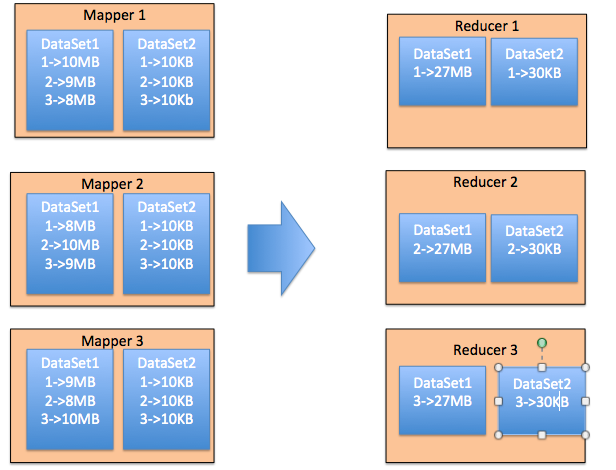
\includegraphics[scale=0.6]{./img/shuffle_join.png}
\caption{Typical Shuffle Join}
\label{fig:shuffle_join}
\end{center}
This figure depicts a typical shuffle join. The mappers have output partitions for two different datasets.
They ensure that all the partitions with the same index get sent to the same reducer. Reducer 1 received partition 1,
Reducer 2 received partition 2, and reducer 3 received partition 3.
\end{figure}

\subsection {Broadcast Join}
The diagram above  may seem to imply that mappers and reducers
are different machines. However, this distinction is artificial and there are no seperate machines for mappers and reducers. 
Therefore, not all data in the shuffle stage is transferred over the network. In Figure~\ref{fig:shuffle_basic}, if Mapper 1
and Reducer 1 were the same machine, the key-value pair A=7 would be read locally and not have to be received over the network.

Because transferring data over the network could be a bottleneck, the broadcast join tries to increase the amount of data 
being read locally \cite{sparkanalysis}. For instance, in Figure~\ref{fig:shuffle_join}, Dataset 1 is drastically bigger than Dataset 2. As seen in Figure~\ref{fig:broadcast_join},
the broadcast join keeps the bigger dataset in place and sends the entirety of Dataset 2 to every reducer. Even though all of Dataset 1 stays in place, this method will still find all intersections beteen the datasets  because all partitions of Dataset 2 are sent to every reducer. The diagram shows that only Dataset 2 is transferred and thus the  network traffic is reduced from megabytes to kilobytes.

Broadcast Join is not always the optimal strategy. Because the entirety of the smaller dataset is sent to every partition, the amount of total computation time increases. Additionally, if the datasets are approximately the same size, network traffic will actually increase. 
Each join strategy is the optimal strategy in different situations. Thus, it becomes imperative
to pick the strategy after the mappers have run and the size of the map output partitions is known.

 \begin{figure}[h]
\begin{center}
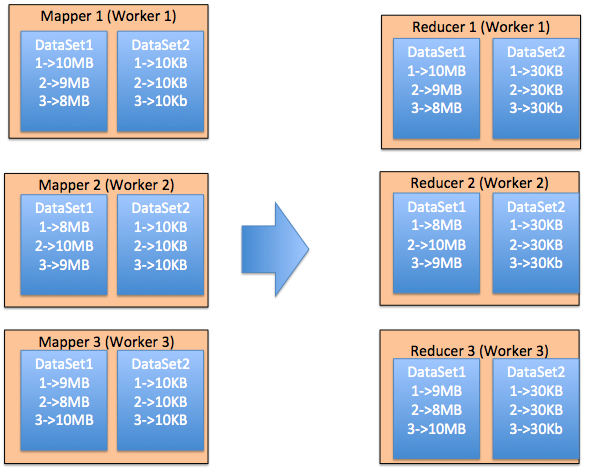
\includegraphics[scale=0.6]{./img/broadcast_join.png}
\caption{Broadcast Join}
\label{fig:broadcast_join}
\end{center}
This figure depicts a Broadcast Join. As evidenced, the bigger dataset stays entirely in place but the entirety 
of the smaller dataset is sent to the each reducer. This cuts network traffic from megabytes to kilobytes.
\end{figure}


